%!TEX root = ../dissertation.tex
\begin{savequote}[75mm]
Knowledge knows no bounds.
\qauthor{Creator}
\end{savequote}

\chapter{Motivation for searches beyond the Standard Model}
%\newthought{There's something out there that we don't know.} 

\section{The Standard Model and the Higgs Boson}
\paragraph{}
The Standard Model(SM) has been the best description of the microscopic world ~\cite{Griffiths,Tully,Pdg,Schwartz}. 
The SM consist of fermions (spin $\frac{1}{2}$) and bosons (spin $1$) as shown in Figure ~\ref{fig:SM}, which interact through: electromagnetism (EM), the strong nuclear force and the weak nuclear force. 
Fermions are the basic building blocks of matter, which consists of three generations of Leptons ($e$, $\mu$, $\tau$, $\nu_e$, $\nu_{mu}$, $\nu_{tau}$) and quarks ($u$, $d$, $c$, $s$, $t$, $b$). 
They all interact iva the weak force. In addition, the charged leptons and quarks interact via the EM force and the quarks also interact via the strong force. 
Bosons are force mediators. EM force mediates through the photon $\gamma$, the strong force meidates through the gluon $g$, and the weak force mediates through $W^{\pm}$ and $Z$ bosons.

\begin{figure}[h!]
  \centering
  \captionsetup{justification=centering}
  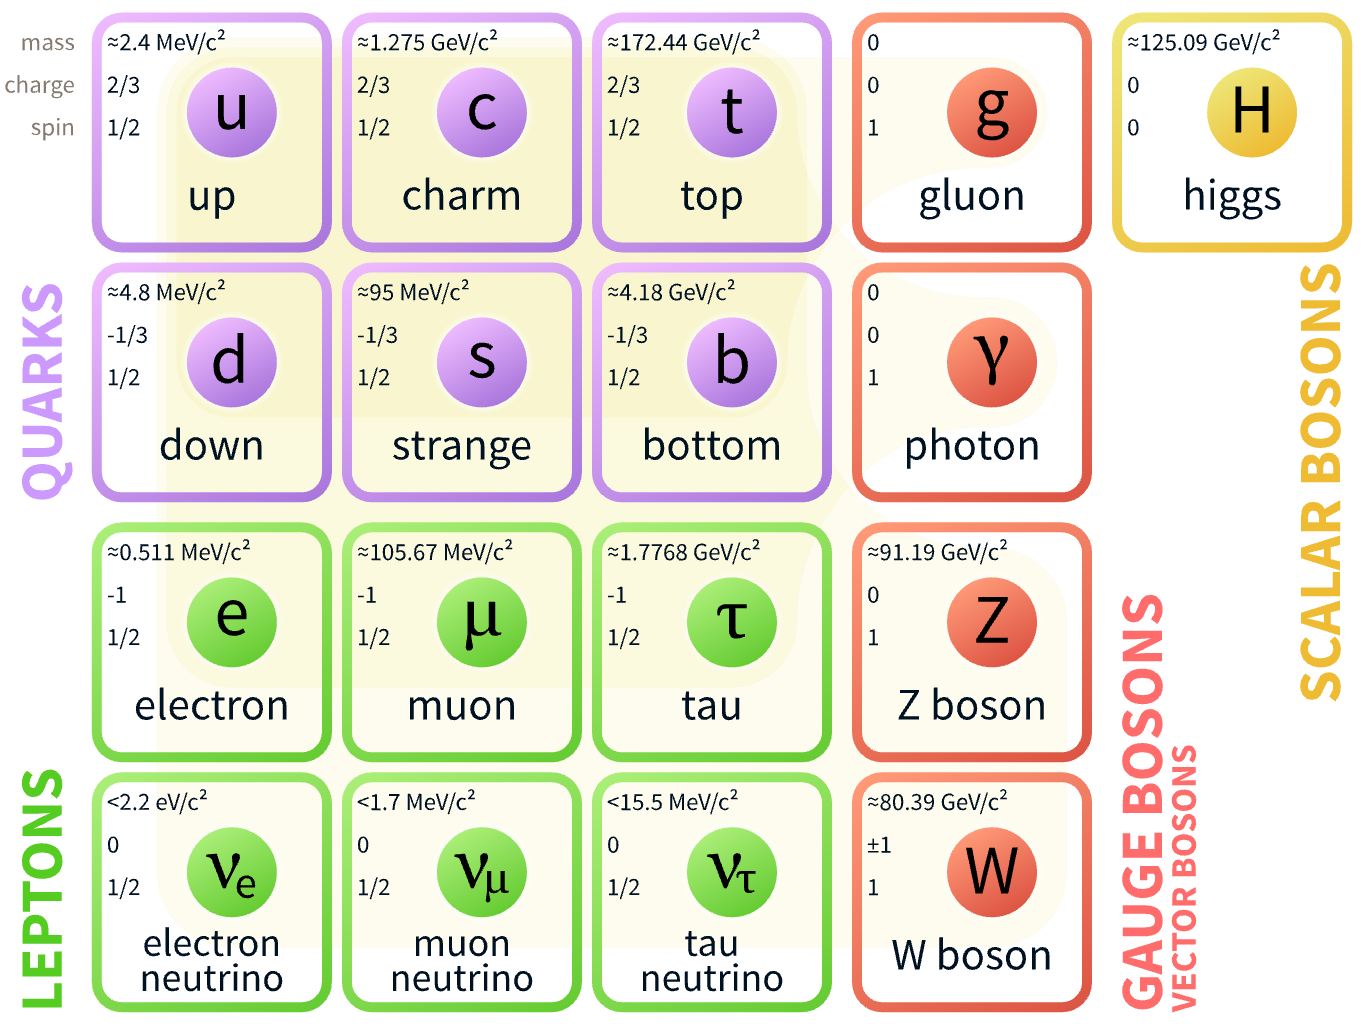
\includegraphics[width=0.6\textwidth]{figures/theory/SM}
  \caption{Fermions and bosons of the Standard Model and their properties~\cite{Pdg}.}
  \label{fig:SM}
\end{figure}

\paragraph{}
However, in SM, due to the gauge invriance under $SU(2)_{L}$, fermions have to be massless in order to have pure left handed states. The bosons must also be massless as required by the gauge principle. The Higgs mechanism introduces a scalr Higgs field with nonzero vaccum expectation values, which impledes and interacts with the propagation of gague bosons and fermions, hence gives them valid mass terms~\cite{Tully}. This broken symmetry of the Standard Model predicts the extra particle degree of freedom as the Higgs boson. The terms inside the Higgs potential are shown in equation~\ref{eqn:higgspotential}.

\begin{equation}
\label{eqn:higgspotential}
V(\phi_{H}) = \lambda \nu^2 \phi_{H} ^2  + \lambda \nu \phi_{H} ^3  + \frac{1}{4}\lambda \phi_{H} ^4 
\end{equation}

where $\nu$ corresponds to the vaccum expectation value of the field, determined to be around $246$ \GeV. The first term gives the Higgs mass, as $ \sqrt{2\lambda}\nu$, measured to be $125.09 \pm 0.24$ \GeV. Hence all parameters in this potential is known. The second term provives an $hhh$ vertex, which corresponds to the trilinear coupling of the Higgs boson. This means that in SM, a two Higgs production (di-Higgs) can happen through a single Higgs.

Add more from \href{http://pdg.lbl.gov/2017/reviews/rpp2016-rev-higgs-boson.pdf}{here}.



\section{Di-Higgs in the Standard Model}
\paragraph{}
There has been many literatures about modifications of Higgs self coupling. Using standard model measurements and their precisions, we can constrain the self coupling parameter to an order of magnitude, see \href{https://arxiv.org/abs/1702.07678}{note}.


\section{Di-Higgs in Beyond the Standard Model Physics}


\section{Di-Higgs Decay and search perspectives}

%\paragraph{}CMS latest search result on di-Higgs is also included \href{https://arxiv.org/pdf/1708.08249.pdf}{here}.